\chapter{Introduction}
\graphicspath{{Chapter1/Figs/}{Chapter1/Figs/}}

\section{Background}
\label{chapter1-background}

There has been a long-standing interest in developing neural interfaces, systems that sense electrical impulses from the nervous system and use them to intercommunicate with the human brain. Successful research into the development of technologies that enable neural interfaces has been going on for decades \citep{vidal_real-time_1977}. Progress has accelerated significantly in the past few years, especially since the advent of modern processing capabilities such as in deep learning with convolutional neural networks (CNN) or generative adversarial networks (GAN) \citep{gonfalonieri_deep_2019}. In particular, a related discipline called brain-computer interfacing (BCI), a field focused on the direct interaction between brains and computers, has accumulated much momentum since the popularity of companies like Neuralink and Kernel.

One aspect of neural interfaces is hardware tailored to the human body. Whether it is an invasive sensor, such as in electrocorticography (ECoG), a method which uses electrodes placed on the surface of the brain, or a non-invasively placed sensor on the body, such as in electroencephalography (EEG). Both methods measure electrical activities produced by neurons; however, with decreasing spatial precision, the farther the electrode is placed from the brain, the more body structures (e.g. bones) are between firing neurons and the measuring sensor. The other aspect is software that reads and interprets data of these hardware sensors. Both aspects present their own set of challenges and complexities. Nonetheless, complete and applicable neural interfaces work in practice and have been used for many years in patients with neurological disorders \citep{braingate_publications_nodate}. There are also consumer and non-clinical neural interfaces available, such as the Neurosity and OpenBCI products, which aim to democratise the use of EEG sensors by offering low-cost hardware and simple-to-use software.

This thesis will focus on the software aspect of non-invasive neural interfaces and the challenges and complexities that arise in the given context of modern software engineering for production-ready end-user facing brain-computer interface applications.

\nomenclature[cnn]{CNN}{Convolutional neural networks}
\nomenclature[gan]{GAN}{Generative adversarial networks}
\nomenclature[bci]{BCI}{Brain-computer interface}
\nomenclature[ecog]{ECoG}{Electrocorticography}
\nomenclature[eeg]{EEG}{Electroencephalography}

\section{Relevance}
\label{chapter1-relevance}

\begin{figure}
  \centering
  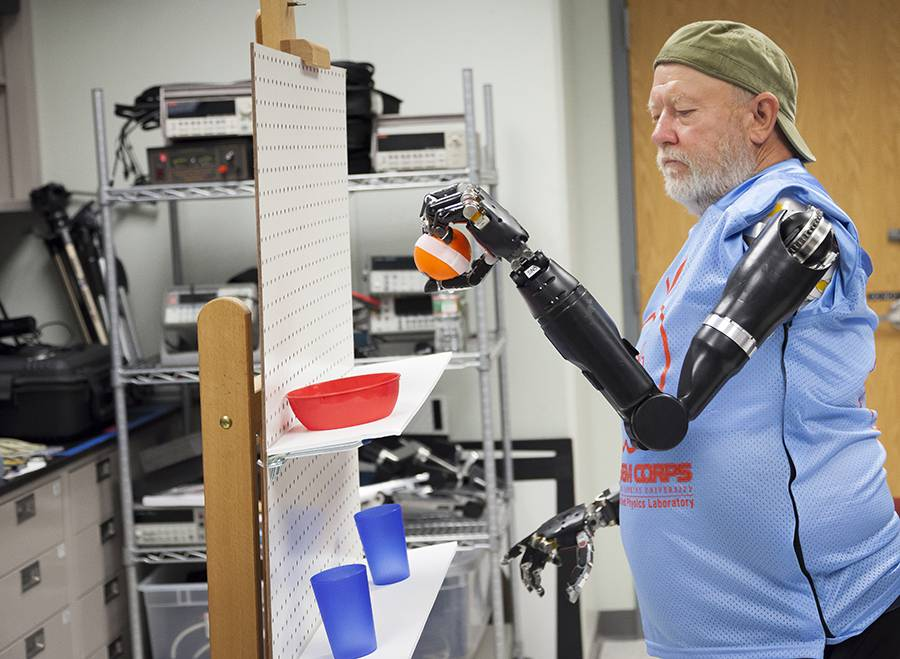
\includegraphics[width=\linewidth]{prostetic-arms.jpg}
  \caption{Les Baugh, an amputee, is using a neural interface to control two robotic arms with his thoughts \citep{campbell_amputee_2014}.}
  \label{fig:prostetic-arms}
\end{figure}

The possibilities of connecting the human brain with computers are almost limitless because one has to imagine that we are the brain, that our own perception of the world, all our feelings, thoughts and actions are supposed to be contained in the electrical impulses of our brain. The ability to communicate directly with our thoughts and the outside world — whether through digital or physical objects — is a fantastic prospect. There are several use cases: Controlling prosthetic limbs for amputees \citep{murphy_electroencephalogram-based_2017}, communication for people with locked-in syndrome \citep{chaudhary_spelling_2022}, diagnosing neurological problems and improving the mental capacities of elderly patients \citep{belkacem_brain_2020} are promising examples, to name a few.

It may appear evident that neural interfaces can significantly impact the field of therapeutics and accessibility for a small subset of the human population. However, one can envision not only alleviating deplorable living conditions but also improving the lives of healthy people through more natural or efficient ways of interacting or by directly altering human brains themselves. Because most current neural interface applications concentrate on the first aspect of therapeutics and accessibility, other use cases, such as stimulating the brain to improve concentration, modifying cognitive load, or even uploading new knowledge directly into the brain, may appear to be science fiction ideas.

Regardless, many intelligent people — research labs or even entire companies — are developing neural interface hardware and software aimed at the general population without conditions that envision a future for such use cases in the long term. The applicability of a neural interface system to the mainstream will depend on several factors, presumably an important factor of which is the hardware's form factor. Nonetheless, the totality of the ecosystem in which the software resides is a valuable aspect that should not be overlooked.

\section{Research question}
\label{chapter1-research-question}

\begin{figure}[ht]
  \centering
  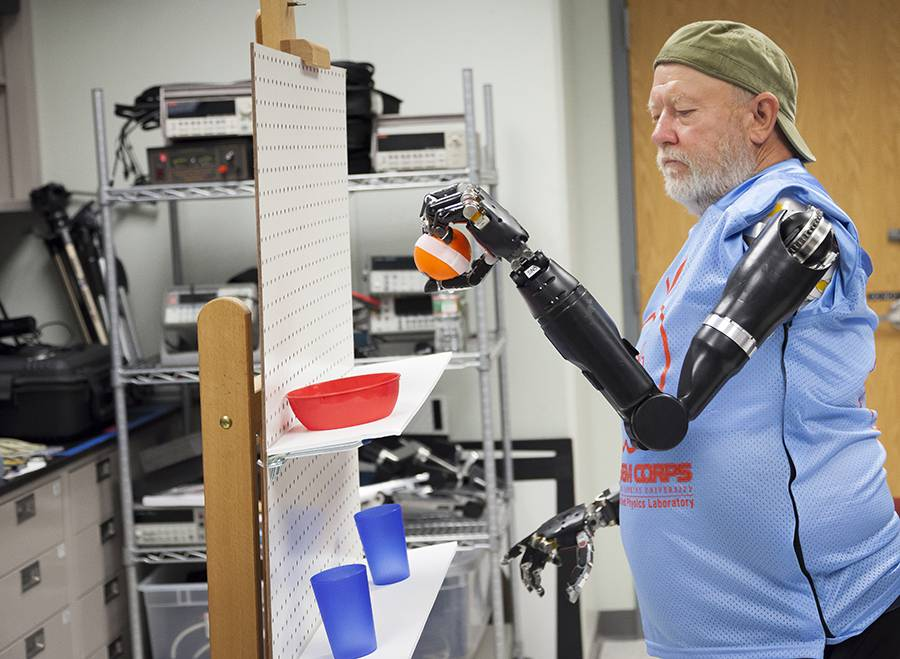
\includegraphics[width=\linewidth/2]{prostetic-arms.jpg}
  \caption{Difference between a bi-directional and uni-directional neural interface and its software components (own representation, 2022).}
  \label{fig:directional-system}
\end{figure}

Whether it is a bidirectional and invasive neural interface with the potential to be implanted on a large scale, as e.g. Neuralink is aiming to do, or a unidirectional and non-invasive interface in various form factors that are also aimed at the mass market, such as in a pair of glasses or a pair of headphones, the data collected from the brain would always need to be processed, contextualised, and classified to produce an intelligible output — be it in real-time or deferred processing. The research question of the present article is on determining what technical components such a software system would require to be production-ready and suitable for a mass-market product. The emphasis is on a holistic view of such a system, which means that the entire technology stack is taken into account in answering the research question.

Furthermore, most current neural interface software systems in production, for example, for an interface implanted in a living patient, are typically run in a local environment, i.e. the software system and its components are typically located on a physically nearby computer, usually connected by a cable, to reduce latency and avoid complexities introduced by a wireless protocol. There is already interesting research on wireless mobile brain-computer interfaces (mBCI) by \citeauthor{minguillon_mobile_2017} \citeyearpar{minguillon_mobile_2017} or possible implications of human brain/cloud interfaces (B/CI) by \citeauthor{martins_human_2019} \citeyearpar{martins_human_2019}, which analyses bringing future large-scale neural software systems into the cloud.

\nomenclature[mbci]{mBCI}{Mobile brain-computer interface}
\nomenclature[bc-i]{B/CI}{Brain/cloud interface}

% Goal 1: State your research question
% - The goal of the present article is to…
% - The research question of the present article is…
% Goal 2: State your hypotheses/ predictions
% - We hypothesize that…
% - We predict that…
% - Two hypotheses are conceivable…
% - Our primary hypothesis is that…
% - Drawing on theory X, we hypothesize that…
% Goal 3: Give a rough outline of your research
% - We tested whether patients with a diagnosed major depression would report less depressive
% feelings after treatment X compared to a placebo treatment.
% - To test this hypothesis, we ….
% - To answer this question, we …
% - For this purpose, we conducted three studies. First,… Second,… Third,…
% - To shed more light on this, we used a combination of computer simulations and empirical
% studies. First, we used computer simulations to determine what behaviour would arise if theory
% 3
% X is true and what behaviour would arise if theory Y was true. Next, we tested these two
% predictions in three empirical studies.
% - The present article consists of three sections. In section 1, … In section 2,… In section 3

\section{Goals}
\label{chapter1-goals}

% o Does your introduction go from broad (topic) to specific (your research)?
% o Did you make clear why your topic is important?
% o Did you describe just enough research so that readers can understand how your
% research is the next logical step?
% o Did you make clear how your research is novel?
% o Did you make clear what is speculation, and what are established facts?
% o Did you add citations for everything you present as facts?
% o Did you use common scientific jargon?
% o Did you explain the jargon you use?